
\clearpage
\refstepcounter{PagePtr}\label{P:scraping}
\section{スクレイピング}
クレイピングとは、ウェブページから情報を取り出すことをいいます。
スクレイピングの手順はウェブページをダウンロードして、ウェブページから欲しい情報を探して取り出し、そして、取り出し情報を加工します。
\ref*{E:CURL},\ref*{E:HTML}
で手動でウェブページをダウンロードして、そこから情報を取り出しました。
そのあとの\ref*{E:SCRAPING}では、同じ手順をプログラムで自動で行いました。
ウェブページから取り出した情報をプログラムから\ruby{有効的}{ゆうこうてき}に使う方法を学びましょう。
ウェブページから取り出した情報をもとにセンサーを使ったり、情報をウェブページに\ruby{反映}{はんえい}することもできます。
ウェブページから\ruby{価値}{かち}のある情報を取り出して、今まで習った\ruby{技術}{ぎじゅつ}と組み合わせて役に立つプログラムを作れるように考えながら例題を進めていきましょう。



\bigskip
\refstepcounter{Exercise}
\clearpage\section{\theExercise アメダスのウェブページをスクレイピングする}
\addtocounter{Exercise}{-1}\refstepcounter{Exercise}\label{E:amedas}
%\newline
考え方

まずは、ウェブブラウザでアメダスのページを見てみよう。
授業で使用したホームページを開いてください。
\textbf{({\textasciitilde}/08/links.html)}

アメダスをクリックします。



\begin{center}
  % Unhandled or unsupported graphics:
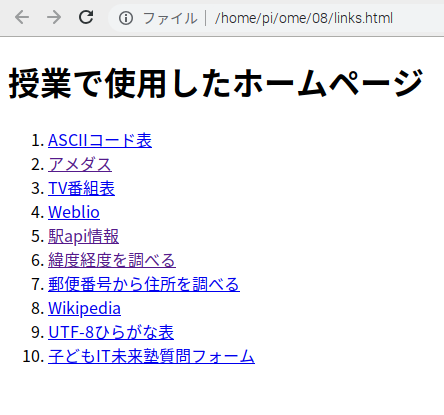
\includegraphics[width=0.55\textwidth]{./text08-img/textbook-img017.png}

\end{center}



アメダスのウェブページが開きます。

\begin{center}
  % Unhandled or unsupported graphics:
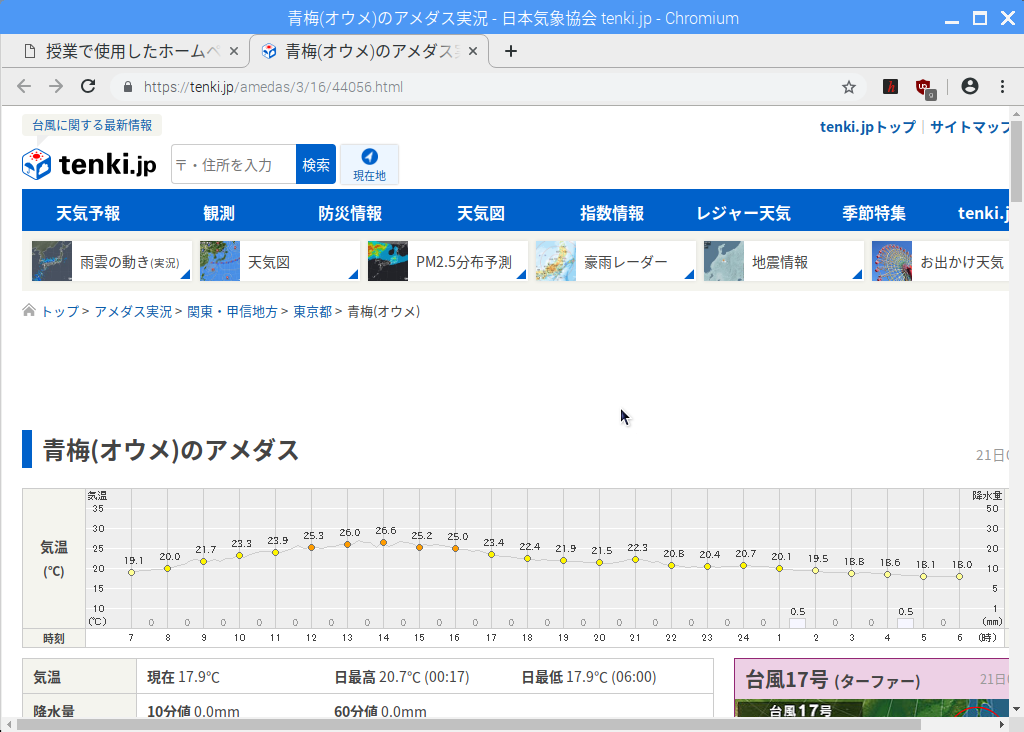
\includegraphics[width=0.9\textwidth]{./text08-img/textbook-img028.png}

\end{center}
\clearpage
少ししたのほうに”アメダス\ruby{履歴}{りれき}(10分観測値)”という見出しがあります。

青梅市のアメダス観測データを10分毎に表にしたものです。



\begin{center}
  % Unhandled or unsupported graphics:

\includegraphics[width=0.9\textwidth]{./text08-img/textbook-img029.png}

\end{center}
今回はこの表から最新の10分観測値の情報を自動でプログラムから取得して、さらに取得した情報をプログラムで利用します。



\begin{center}
  % Unhandled or unsupported graphics:
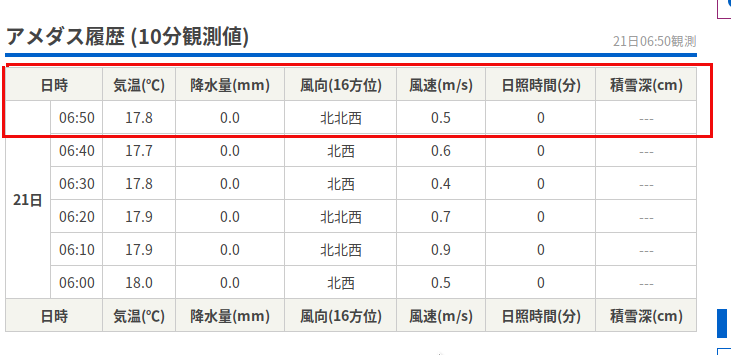
\includegraphics[width=0.9\textwidth]{./text08-img/textbook-img029-1.png}

\end{center}

\bigskip

\clearpage
まずはプログラムを動かしてみましょう。

ターミナルを開いて

hsed

と実行します



\begin{center}
  % Unhandled or unsupported graphics:
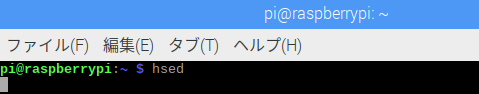
\includegraphics[width=0.8\textwidth]{./text08-img/textbook-img013.png}

\end{center}

\bigskip


\bigskip


\bigskip

HSPスクリプトエディタが開くので

ファイル → 開く..

をクリックして\textbf{{\textasciitilde}/08/amedas.hsp}を開きます。

プログラムが表示されます。



\begin{center}
  % Unhandled or unsupported graphics:
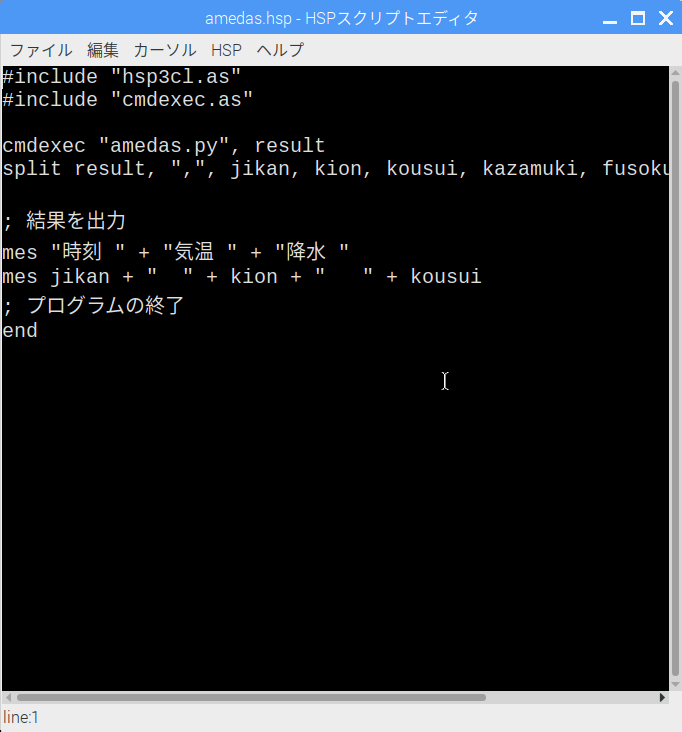
\includegraphics[width=0.8\textwidth]{./text08-img/textbook-img030.png}

\end{center}

\bigskip


\clearpage
F5を押して実行してみましょう。実行結果はターミナルに表示されます。



\begin{center}
  % Unhandled or unsupported graphics:
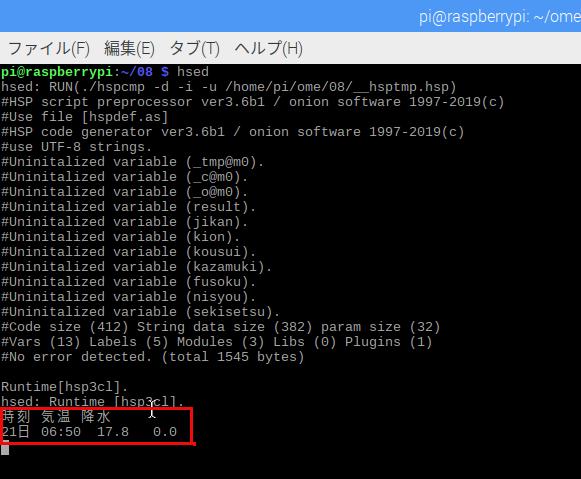
\includegraphics[width=0.9\textwidth]{./text08-img/textbook-img031.png}

\end{center}

\bigskip


表示されている\ruby{時刻}{じこく}、気温、降水とブラウザで見たアメダスの情報を\ruby{比}{くら}べてみてください。



\begin{center}
  % Unhandled or unsupported graphics:
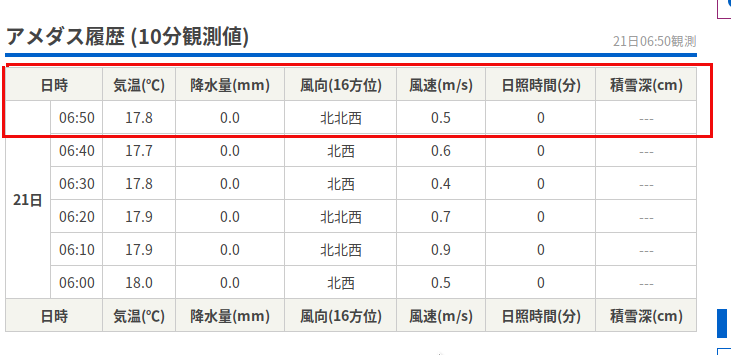
\includegraphics[width=0.9\textwidth]{./text08-img/textbook-img029-1.png}

\end{center}
同じ値が表示されています。
このようにHSPのプログラムでウェブページからアメダスの情報を取得することができました。



\clearpage
プログラム解説

この例題プログラムでは、amedas.pyというコマンドを使って、ウェブページからアメダスの情報を取得しています。

% \begin{center}
% \begin{boxedminipage}{17.126cm}
% \begin{enumerate}
% \baselineskip 10pt
% \setlength{\itemsep}{0cm} % 項目間
% \item \#include {\textquotedbl}hsp3cl.as{\textquotedbl}
% \item \#include {\textquotedbl}cmdexec.as{\textquotedbl}
% \item
% \item cmdexec {\textquotedbl}amedas.py{\textquotedbl}, result
% \item split result, {\textquotedbl},{\textquotedbl}, jikan, kion, kousui, kazamuki, fusoku, nisyou, sekisetsu
% \item
% \item ; 結果を出力
% \item mes {\textquotedbl}時刻 {\textquotedbl} + {\textquotedbl}気温 {\textquotedbl} +
% {\textquotedbl}降水 {\textquotedbl} \
% \item mes jikan + {\textquotedbl} \ {\textquotedbl} + kion + {\textquotedbl} \ \ {\textquotedbl} + kousui
% \item ; プログラムの終了
% \item end
% \end{enumerate}
% \end{boxedminipage}
% \end{center}


\begin{table}[htbp]
    \centering
    % \caption{文字タイプ表}
    \begin{tabular}{|l|}
        \hline
        
        1. \#include {\textquotedbl}hsp3cl.as{\textquotedbl}\\
        2. \#include {\textquotedbl}cmdexec.as{\textquotedbl}\\
        3. \\
        4. cmdexec {\textquotedbl}amedas.py{\textquotedbl}, result\\
        5. split result, {\textquotedbl},{\textquotedbl}, jikan, kion, kousui, kazamuki, fusoku, nisyou, sekisetsu\\
        6.\\
        7. ; 結果を出力\\
        8. mes {\textquotedbl}時刻 {\textquotedbl} + {\textquotedbl}気温 {\textquotedbl} + {\textquotedbl}降水 {\textquotedbl} \ \\
        9. mes jikan + {\textquotedbl} \ {\textquotedbl} + kion + {\textquotedbl} \ \ {\textquotedbl} + kousui\\
        10. ; プログラムの終了\\
        11. end\\
        
        \hline
    \end{tabular}
\end{table}



4行目でHSPプログラム内からamedas.pyコマンドを実行しています。

cmdexec命令は、execと\ruby{基本的}{きほんてき}には同じですが、実行するコマンドの後に変数名をつけます。
この変数にはコマンドの実行結果が文字列で入ります。

一度、amedas.pyコマンドをターミナルで実行してみましょう。
ターミナルを開きます。

amedas.py を実行します。

カンマ(,)で区切られて値が表示されています。

\begin{center}
  % Unhandled or unsupported graphics:
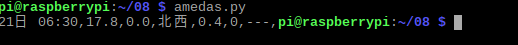
\includegraphics[width=\textwidth]{./text08-img/textbook-img032-1.png}

\end{center}
これらの値がなにを意味しているのか見てみましょう。

\textbf{amedas.py \ {}-{}-print-headers}

を実行します。



\begin{center}
  % Unhandled or unsupported graphics:
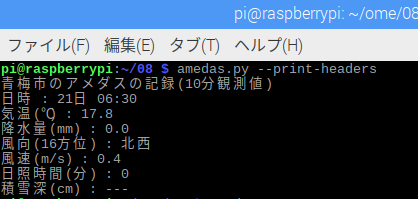
\includegraphics[width=\textwidth]{./text08-img/textbook-img032-2.png}

\end{center}
日時、気温、降水量、風向、風速、日照時間、積雪深の順番で値と値の見出しが表示されています。

このカンマ(,)区切りの数値も同じ\ruby{並}{なら}びで表示されています。

HSPのプログラムに\ruby{戻}{もど}ります。

\begin{center}
  % Unhandled or unsupported graphics:
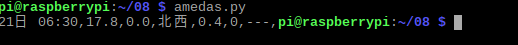
\includegraphics[width=\textwidth]{./text08-img/textbook-img032-1.png}

\end{center}
5行目で、カンマ(,)で区切られた実行結果を分解してそれぞれ変数へいれています。

結果は日時、気温、降水量、風向き、風速、日照、積雪深の順になっているので、

split result, {\textquotedbl},{\textquotedbl}, jikan, kion, kousui, kazamuki, fusoku, nisyou, sekisetsu


\bigskip

% \begin{center}
% \tablefirsthead{}
% \tablehead{}
% \tabletail{}
% \tablelasttail{}
% \begin{supertabular}{|m{16.806cm}|}
% \hline
% split命令の使い方

% split 分解前の変数(文字列), \ “区切り文字”,
% 変数..

% 例 :

% split “りんご,ぶどう,オレンジ”, \ “,”, apple, grape, orange

% \ 文字列を
% カンマ(,)で区切って順番に変数にいれている

% apple ← “りんご”

% grape ← “ぶどう”

% orange ← “オレンジ”\\\hline
% \end{supertabular}
% \end{center}


\begin{table}[htbp]
    \centering
    % \caption{文字タイプ表}
    \begin{tabular}{|l|}
        \hline
        
        split命令の使い方\\

        split 分解前の変数(文字列), \ “区切り文字”,変数..\\
        例 : \\
        split “りんご,ぶどう,オレンジ”, \ “,”, apple, grape, orange\\
        文字列をカンマ(,)で区切って順番に変数にいれている\\

        apple ← “りんご”\\

        grape ← “ぶどう”\\

        orange ← “オレンジ”\\
        \\\hline
    \end{tabular}
\end{table}



\bigskip


\bigskip

変数の順番も対応させます。

日時  → \ jikan

気温  → kion  

降水 → kousui

風向き→ kazamuki

風速 → fusoku

日照 → nisyou

積雪深→ sekisetsu

変数に文字列として入れています。


\bigskip

9行目で日時(jikan), 気温(kion),
降水(kousui)を表示させています。

mes jikan + {\textquotedbl} \ {\textquotedbl} + kion + {\textquotedbl} \ \ {\textquotedbl} + kousui

\refstepcounter{Question}
\clearpage\subsection*{\theQuestion\label{Q:amedas1}}
\begin{itemize}
\item
.例題のプログラムでは、日時、気温、降水だけ表示しています。
		プログラムでは、風向き、風速、日照も取得してます。
		これらも表示させてみましょう。
\end{itemize}
\ \ HINT : それぞれkazamuki, fusoku,
nisyouという変数に情報が入っています。

\refstepcounter{Question}
\subsection*{\theQuestion\label{Q:amedas2}}
\begin{itemize}
\item
kionが25.0度以上のときに、\ruby{現在}{げんざい}の気温を表示し、センサーボードの赤色LEDをつけてみましょう。
		それ以外の場合は、画面に現在の気温を表示し、白色LEDをつけましょう。
\end{itemize}
\ \ HINT :
例題プログラムのkionを数値へ変換してみましょう。

\ \ HINT :
プログラムに応用するには大小の\ruby{比較}{ひかく}とかできると便利です。
大小比較をするには文字列から数値へ変換が必要です

\ \ HSPでは、文字列で表された数値はdouble関数を使って文字列から数値へ変換できます。

\ \ 例えば、



% \begin{center}
% \begin{boxedminipage}{8.326cm}
% \begin{enumerate}
% \baselineskip 10pt
% \setlength{\itemsep}{0cm} % 項目間
% \item kion = “28.2”
% \item kion = double(kion)
% \end{enumerate}
% \end{boxedminipage}
% \end{center}



\begin{table}[htbp]
    \centering
    % \caption{文字タイプ表}
    \begin{tabular}{|l|}
        \hline
        
        1. kion = “28.2”\\
        2. kion = double(kion)
        \\\hline
    \end{tabular}
\end{table}


\bigskip


\bigskip

\refstepcounter{Question}
\subsection*{\theQuestion\label{Q:amedas3}}
\begin{itemize}
\item
このアメダスのスクレイピングの例題とすでに習った技術(センサーボードの使い方、ゲーム、Fabo、赤外線など)と組み合わせるとどんなことができるか考えて、1つ上げてみよう。
\end{itemize}

\bigskip


\bigskip

\clearpage\section{スクレイピングの仕組み}
\ref*{E:SCRAPING}でHSPのプログラムから友達のウェブページのタイトルを取り出したように、スクレイピングでは、HTMLファイルのタグ(\ref*{E:SCRAPING}では{\textless}title{\textgreater}{\textless}/title{\textgreater})を探します。
しかし、ウェブページの欲しい情報はHTMLファイル内のどのタグで作られているでしょうか?ウェブページをダウンロードして、HTMLファイルを\ruby{眺}{なが}めても探しても良いのですが、かなり大変です。
ここでは、ウェブページの欲しい情報がどのHTMLファイル内のどのタグで作られているか調べる方法としてブラウザの\ruby{検証}{けんしょう}ツールを使った方法を紹介します。
アメダスのウェブページを例に試していきます。

\bigskip

まずは、ウェブブラウザでアメダスのページを見てみよう。
授業で使用したホームページを開いてください。
\textbf{({\textasciitilde}/08/links.html)}

アメダスをクリックします。



\begin{center}
  % Unhandled or unsupported graphics:
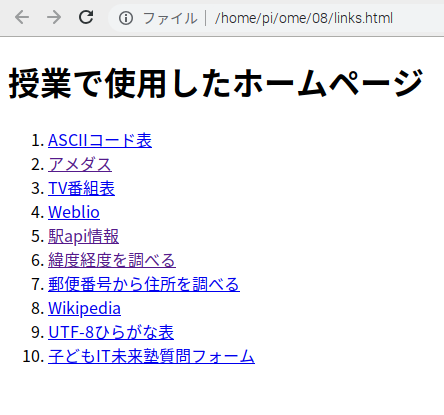
\includegraphics[width=0.5\textwidth]{./text08-img/textbook-img017.png}

\end{center}


アメダスのウェブページが開きます。

\begin{center}
  % Unhandled or unsupported graphics:
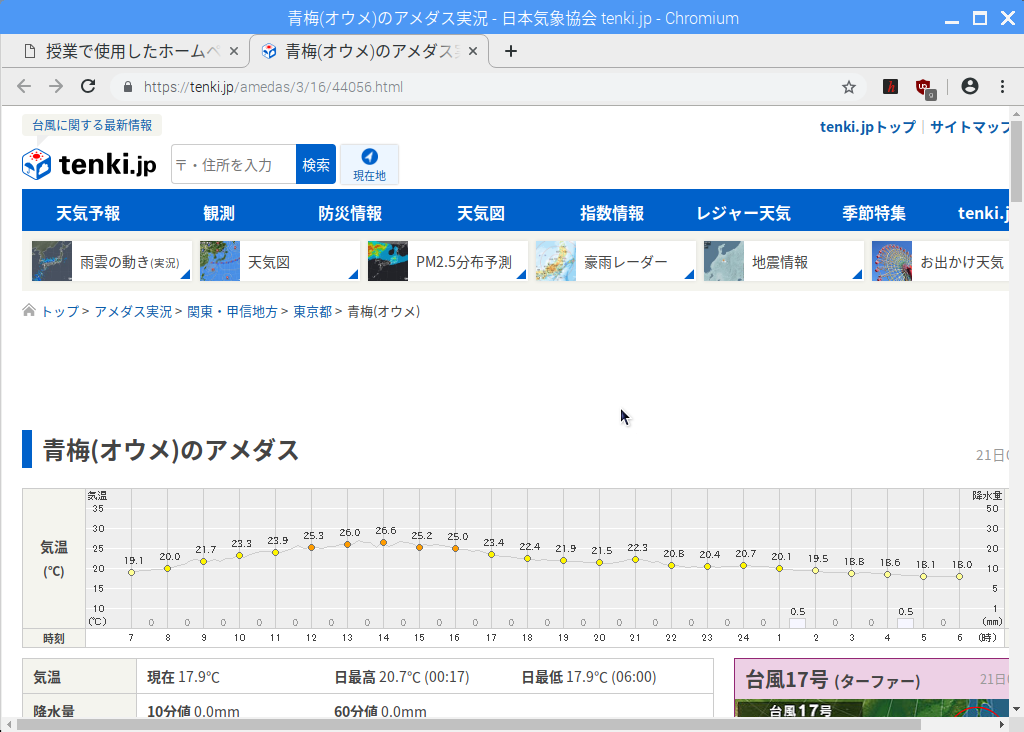
\includegraphics[width=0.7\textwidth]{./text08-img/textbook-img028.png}

\end{center}


\clearpage
少ししたのほうに”アメダス履歴(10分観測値)”という見出しがあります。

青梅市のアメダス観測データを10分毎に表にしたものです。



\begin{center}
  % Unhandled or unsupported graphics:
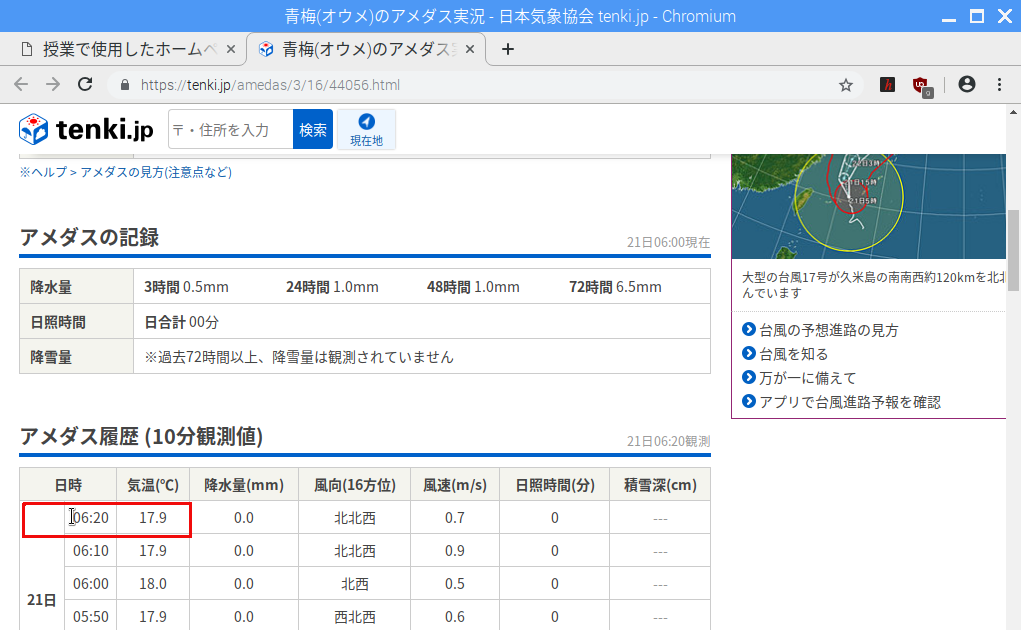
\includegraphics[width=0.8\textwidth]{./text08-img/textbook-img033.png}

\end{center}
10分観測値の表の一番上の行にある、時刻にカーソルを合わせます。
ウェブページを開いた時間によって、表示が変わりますので、値が違っても気にしないでください。

カーソルを合わせたら、左クリックして、メニューを開き、”検証”をクリックします。

\begin{center}
  % Unhandled or unsupported graphics:
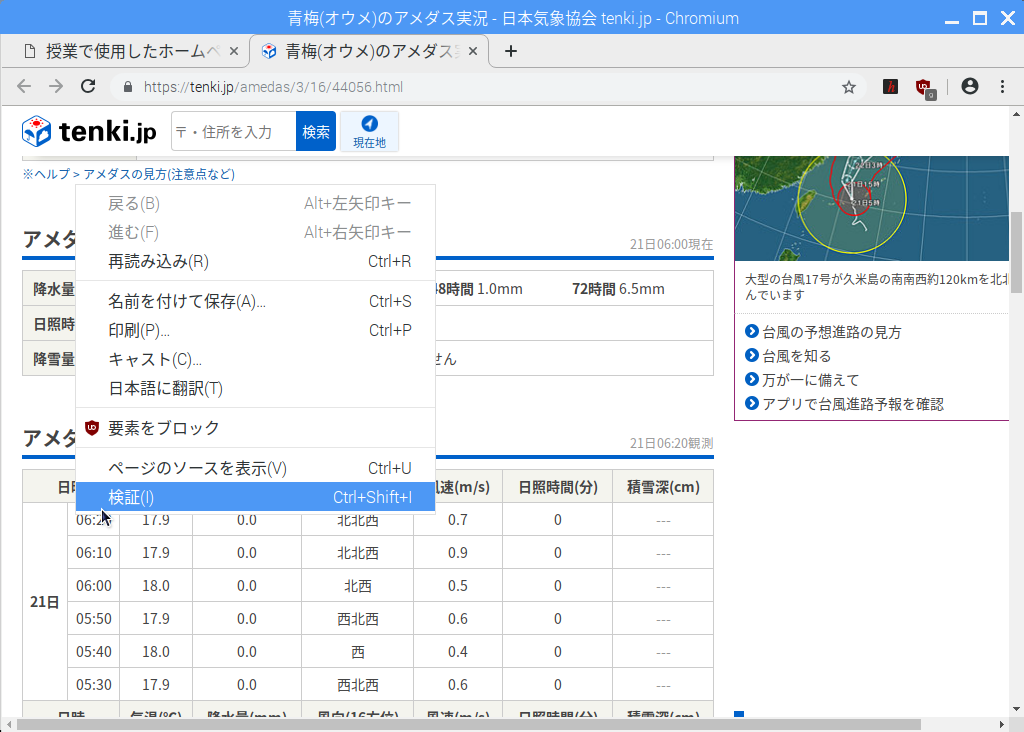
\includegraphics[width=0.8\textwidth]{./text08-img/textbook-img034.png}

\end{center}
\clearpage
検証をクリックすると検証ツールが開きます。



\begin{center}
  % Unhandled or unsupported graphics:
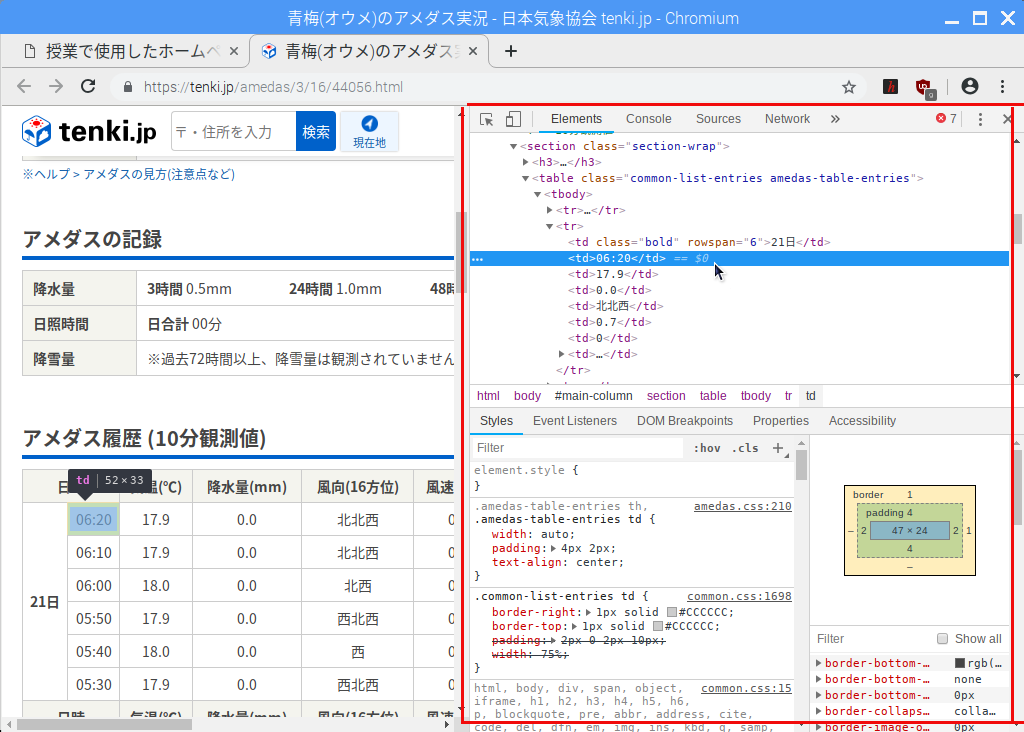
\includegraphics[width=0.9\textwidth]{./text08-img/textbook-img035.png}

\end{center}
検証ツールにはウェブページのHTMLが上半分に表示されています。
現在、カーソルが乗っている(青くなっている)行に対応するウェブページが青く色づけされています。



\begin{center}
  % Unhandled or unsupported graphics:
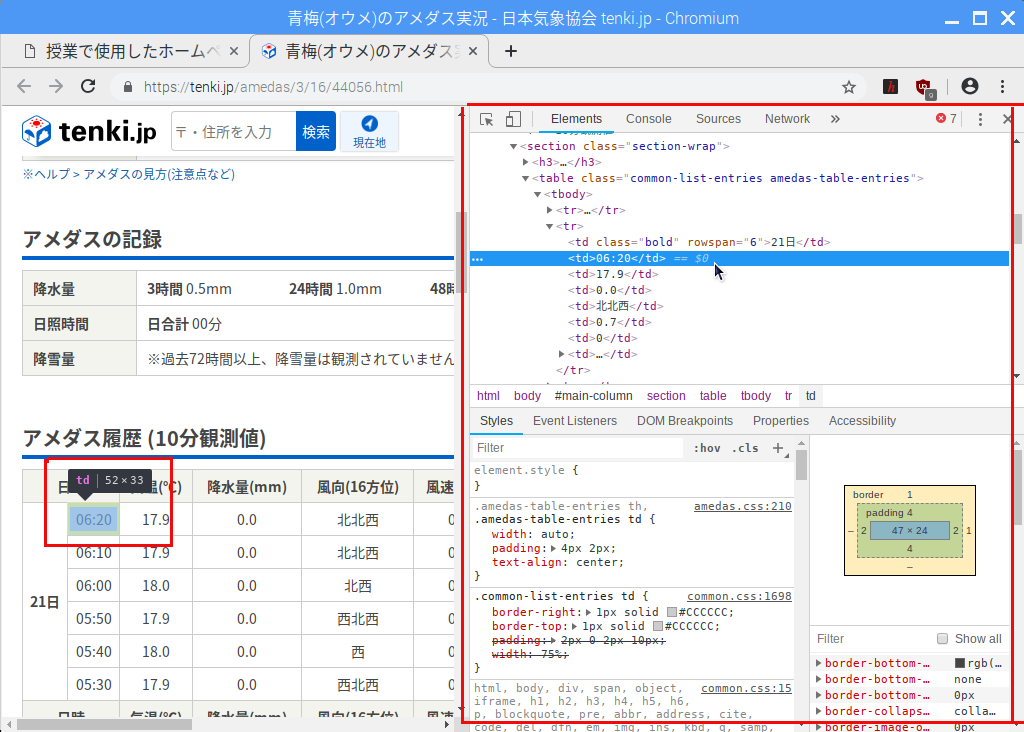
\includegraphics[width=0.9\textwidth]{./text08-img/textbook-img035-2.png}

\end{center}
現在、\ruby{選択}{せんたく}しているのは{\textless}td{\textgreater}{\textless}/td{\textgreater}タグです。
{\textless}td{\textgreater}{\textless}/td{\textgreater}タグ(table
data,
表の値)は表の値にあたる部分を書くときに使用します。

{\textless}tr{\textgreater}{\textless}/tr{\textgreater}タグ(table row,
表の行)は表の1行分を書くときに使います。
{\textless}tr{\textgreater}{\textless}/tr{\textgreater}タグの中に{\textless}td{\textgreater}{\textless}/td{\textgreater}タグを入れて、1行分の表の値を表します。


表は{\textless}table{\textgreater}{\textless}/table{\textgreater}タグ(table,
表)で作りました。


アメダスのサイトから情報を取り出す際には、まずは、{\textless}table{\textgreater}{\textless}/table{\textgreater}タグを探して取り出します。
{\textless}table{\textgreater}{\textless}/table{\textgreater}タグを取り出したあと、その中から、{\textless}tr{\textgreater}{\textless}/tr{\textgreater}タグを取り出して、さらに{\textless}td{\textgreater}{\textless}/td{\textgreater}タグを取り出し、実際の値を取り出すということを行っています。


実際に実行しているamedas.pyコマンドはだいたいこのような流れでアメダスのサイトの表から気温などの情報を取り出しています。


\bigskip


\bigskip



\begin{center}
  % Unhandled or unsupported graphics:
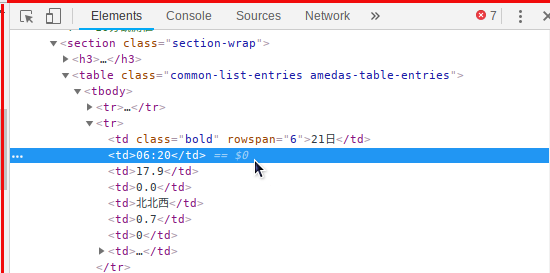
\includegraphics[width=\textwidth]{./text08-img/textbook-img035-3.png}

\end{center}
ちなみに、{\textless}table class=”common-list-entries amedas-table-entries”{\textgreater}

のようにタグに情報がついています。
classはいわば名前のようなもので、このタグについている情報を使ってタグをHTMLファイルから取り出すのが良いです。
このウェブページには、表が何個もあるので、{\textless}table{\textgreater}{\textless}/table{\textgreater}タグだけでは、すべての表が当てはまります。
しかし、このように名前などタグについた情報を\ruby{一緒}{いっしょ}に指定することで、取りたいタグをより\ruby{限定的}{げんていてき}にできます。


\bigskip


\bigskip
\refstepcounter{Exercise}
\clearpage\section{\theExercise amedas.pyをlessで見てみよう}
\addtocounter{Exercise}{-1}\refstepcounter{Exercise}\label{E:amedasLess}
「スクレイピングの仕組み」では、アメダスのウェブページからアメダス観測値を取得する流れを解説しました。
実際にウェブページから値を取り出すのに使用しているコマンド(プログラム)を見てみましょう。
amedas.pyコマンドはHSPのプログラムから\ruby{呼}{よ}び出しているものです。

このプログラムはPython
3(パイソン)という言語で書かれています。
HSPとは書き方が違うので少し\ruby{難}{むず}しいかもしれないですが、プログラムの\ruby{内容}{ないよう}が理解できなくても、問題はないので気楽に見てみましょう。


\bigskip

amedas.pyコマンドもHSPのプログラムと同じくテキストファイルとして記述されています。

まずは、amedas.pyコマンドをlessコマンドで開きます。


\bigskip

\textbf{less /usr/local/bin/amedas.py}



\begin{center}
  % Unhandled or unsupported graphics:
  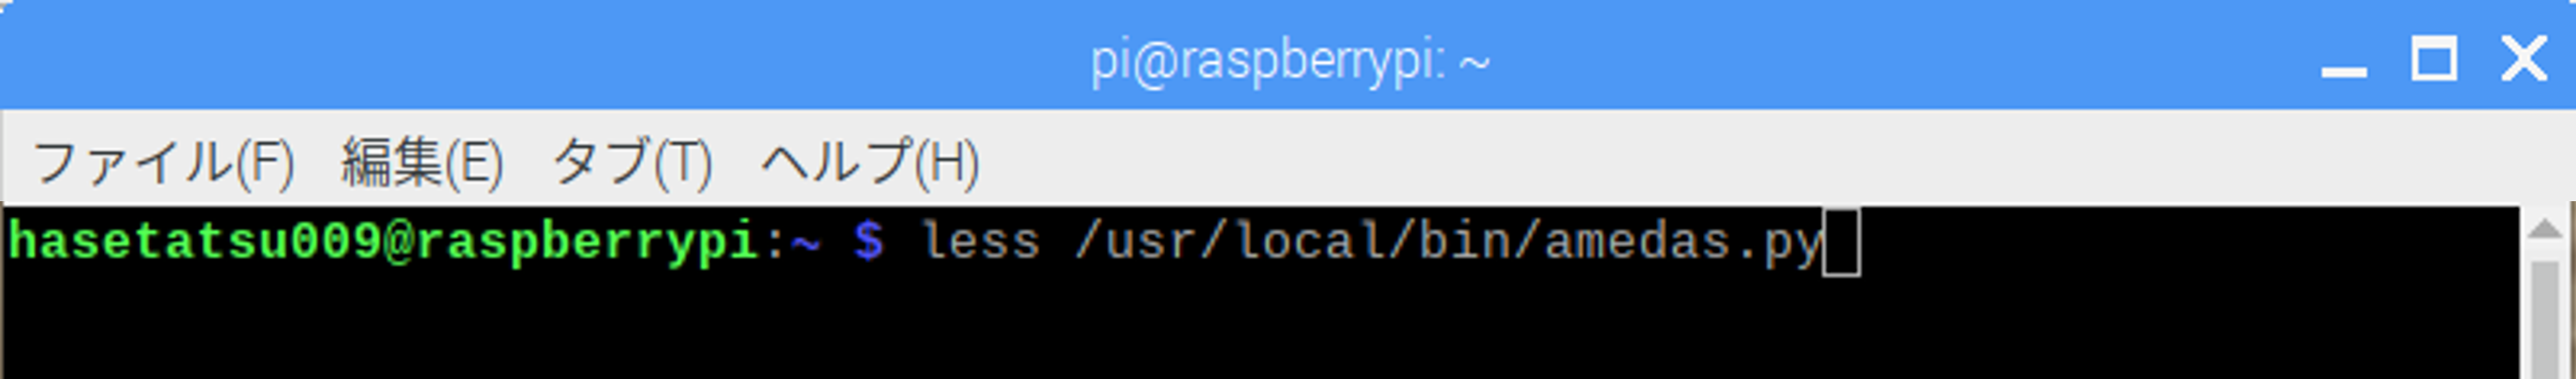
\includegraphics[width=17.006cm,height=2.067cm]{./text08-img/img00036.png}

\end{center}
\begin{center}
  % Unhandled or unsupported graphics:
  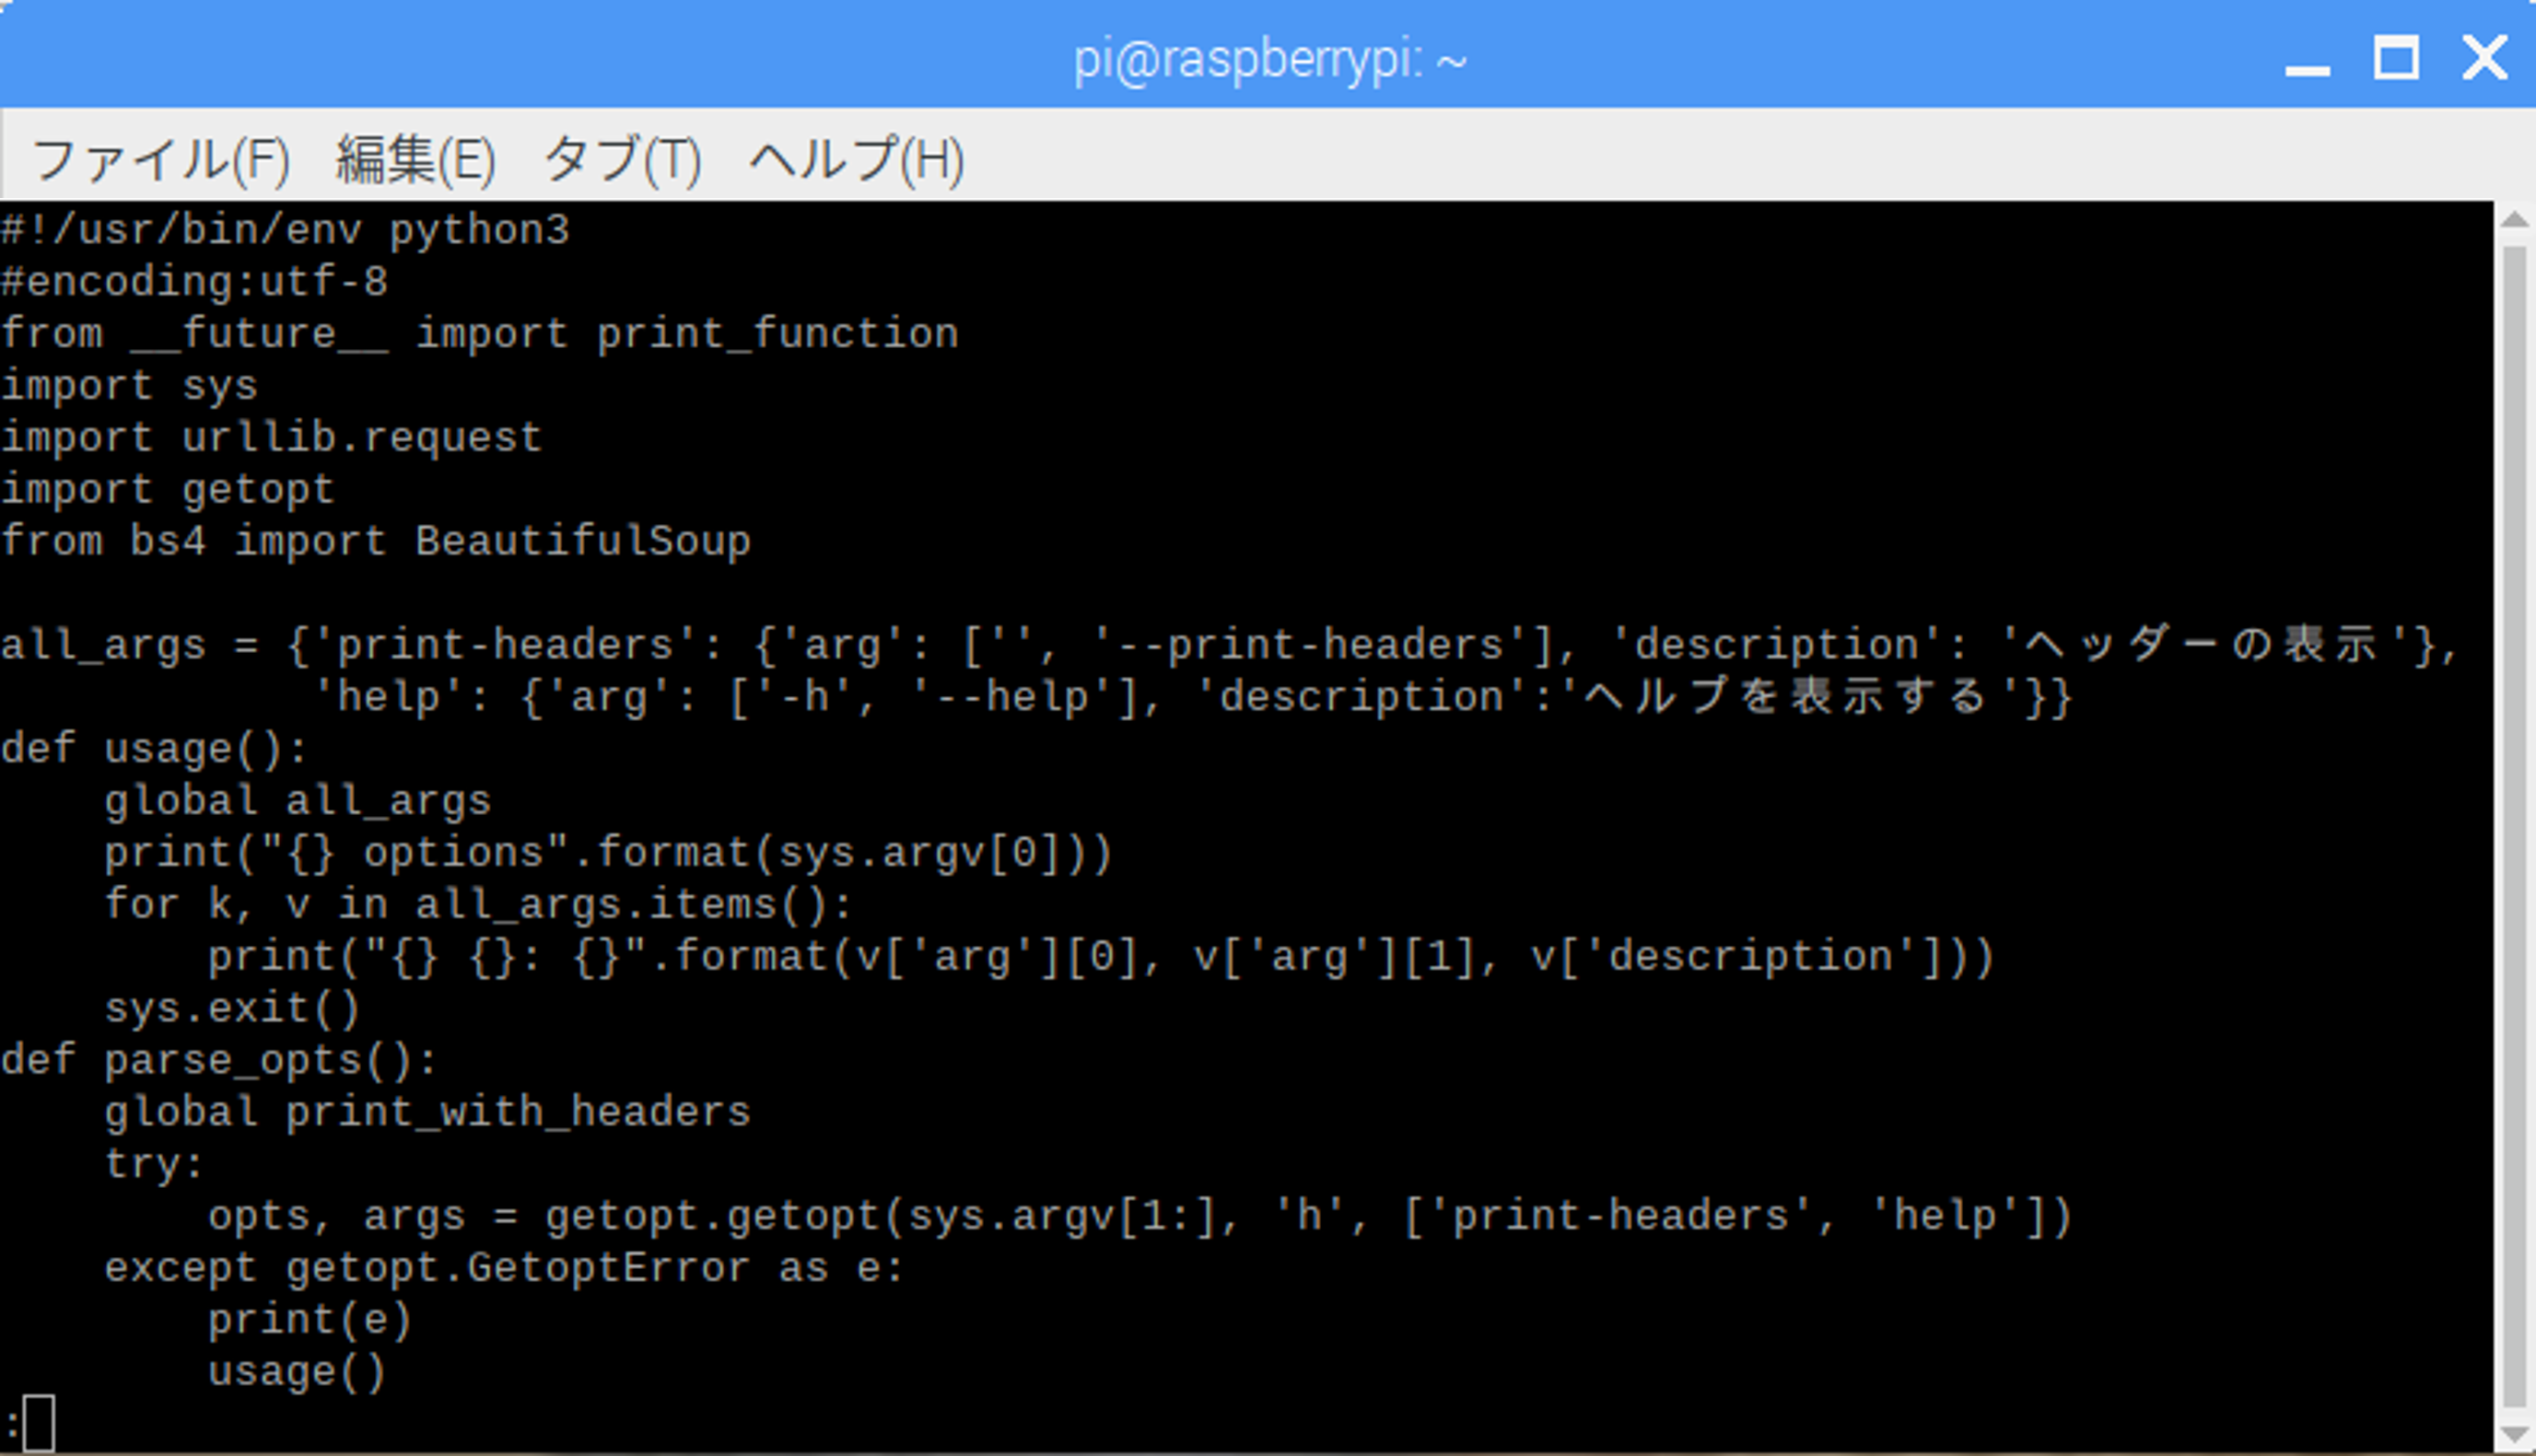
\includegraphics[width=17.006cm,height=9.086cm]{./text08-img/img00037.png}

\end{center}
{\bfseries
(lessコマンドの詳しい使い方は3回目の教科書「2.2.12
ファイルの中身を見てみよう(2)」を見てください)%
%来年度、2.2.12を統一された例題番号へ変更する
%koyaman
%September 23, 2019 8:47 PM
}


\bigskip

\clearpage
実際のスクレイピングの\ruby{処理}{しょり}は30行目から下です。

34行目でhtmlを取得しています。

% \begin{center}
% \begin{boxedminipage}{16.947cm}
% \begin{enumerate}
% \setlength{\itemsep}{0cm} % 項目間
% \setcounter{enumi}{29}
% \item def main():
% \item \ \ \ \ \#アメダスのウェブページのURL
% \item \ \ \ \ url = 'http://tenki.jp/amedas/3/16/44056.html'
% \item \ \ \ \ with urllib.requset.urlopen(url) as response:
% \item  \ \ \ \ \ \ \ html=response.read()
% \item \ \ \ \ parse\_opts()
% \item \ \ \ \ soup = BeautifulSoup(html, 'html.parser')

% %\ \ \ \ …
% \end{enumerate}
% \end{boxedminipage}
% \end{center}



\begin{table}[htbp]
    \centering
    % \caption{文字タイプ表}
    \begin{tabular}{|l|}
        \hline
        
        30. def main():\\
        31. \ \ \ \ \#アメダスのウェブページのURL\\
        32. \ \ \ \ url = 'http://tenki.jp/amedas/3/16/44056.html'\\
        33. \ \ \ \ with urllib.requset.urlopen(url) as response:\\
        34. \ \ \ \ \ \ \ html=response.read()\\
        35. \ \ \ \ parse\_opts()\\
        36 \ \ \ \ soup = BeautifulSoup(html, 'html.parser')\\
        
        \hline
    \end{tabular}
\end{table}


HTMLからタグを探したりするソフトウェア(ライブラリ)にはBeautiful
Soupを使用しています。

37行目では、最初の{\textless}table class={\textquotedbl}common-list-entries
amedas-table-entries{\textquotedbl}{\textgreater}を探して取り出しています。

39行目では、取り出した{\textless}table{\textgreater}タグから{\textless}tr{\textgreater}タグを2行分取り出しています。

44行目で、値の説明(日時、気温、降水などの文字列)

% \begin{center}
% \begin{boxedminipage}{17.658cm}
% \begin{enumerate}
% \setlength{\itemsep}{0cm} % 項目間
% \baselineskip 10pt
% \setcounter{enumi}{36}
% \item \# 最初の{\textless}table class={\textquotedbl}common-list-entries
% amedas-table-entries{\textquotedbl}{\textgreater} ... {\textless}/table{\textgreater}を探す
% \item \ \ \ \ table = soup.find\_all('table', attrs=\{'class' : 'common-list-entries amedas-table-entries'\})[0]
% \item \ \ \ \ \# 2行分取り出す
% \item \ \ \ \ tr = [i for i in table.find\_all('tr')[:2]] \#
% ヘッダー、値の2行
% \item \ \ \ \ result = []
% \item \ \ \ \ for i in tr:
% \item \ \ \ \ \ \ \ \ result.append(i.text.strip())
% \item \ \ \ \ \# 結果をヘッダーと値に分ける
% \item \ \ \ \ headers = [i for i in result[0].splitlines()]
% \item \ \ \ \ data \ \ \ = [i for i in result[1].splitlines()]
% \end{enumerate}
% \end{boxedminipage}
% \end{center}


\begin{table}[htbp]
    \centering
    % \caption{文字タイプ表}
    \begin{tabular}{|l|}
        \hline
        
        37. \# 最初の{\textless}table class={\textquotedbl}common-list-entries amedas-table-entries{\textquotedbl}{\textgreater} ... {\textless}/table{\textgreater}を探す\\
        38. \ \ \ \ table = soup.find\_all('table', attrs=\{'class' : 'common-list-entries amedas-table-entries'\})[0] \\
        39. \ \ \ \ \# 2行分取り出す\\
        40. \ \ \ \ tr = [i for i in table.find\_all('tr')[:2]] \# ヘッダー、値の2行\\
        41. \ \ \ \ result = []\\
        42. \ \ \ \ for i in tr:\\
        43. \ \ \ \ \ \ \ \ result.append(i.text.strip())\\
        44. \ \ \ \ \# 結果をヘッダーと値に分ける\\
        45. \ \ \ \ headers = [i for i in result[0].splitlines()]\\
        46. \ \ \ \ data \ \ \ = [i for i in result[1].splitlines()]\\
        
        \hline
    \end{tabular}
\end{table}






45行目で、値(21日6:20、17.9、0.0など値)

それぞれ{\textless}tr{\textgreater}タグから{\textless}td{\textgreater}の値を取り出しています。


あとは、カンマ(,)区切りで表示しているだけです。
「スクレイピングの仕組み」で説明した流れで実際にプログラムが書かれています。




サンプルプログラム、Pythonのことをもっと詳しく知りたい人はブラウザで

\begin{itemize}
\item Python 3
\item Python 3 スクレイピング
\item Python 3 Beautiful Soup4
\end{itemize}
等を検索してみてください。\\

(※Python 3, Beautiful Soup4(Python
3用)はインストール\ruby{済}{ず}みです)